\section{Thermostat}
\label{proposal}

We present Thermostat, an application-transparent huge-page-aware mechanism to
detect cold pages during execution. The input to Thermostat is a user-specified
tolerable slowdown (3\% in our evaluation) incurred as a result of Thermostat's 
monitoring and due to accesses to data shifted to slow memory. Thermostat periodically
samples a fraction of the application footprint and uses a page poisoning technique
to estimate the access rate to each page with tightly controlled overhead. The
estimated page access rate is then used to select a set of pages to
place in cold memory, such that their aggregate access rate will not result in 
slowdown exceeding the target
performance degradation.  These cold pages are then continually monitored to
detect and rapidly correct any mis-classifications or behavior changes.
In the following sections, we describe the Thermostat in more detail.

\begin{figure*}[t]
\centering
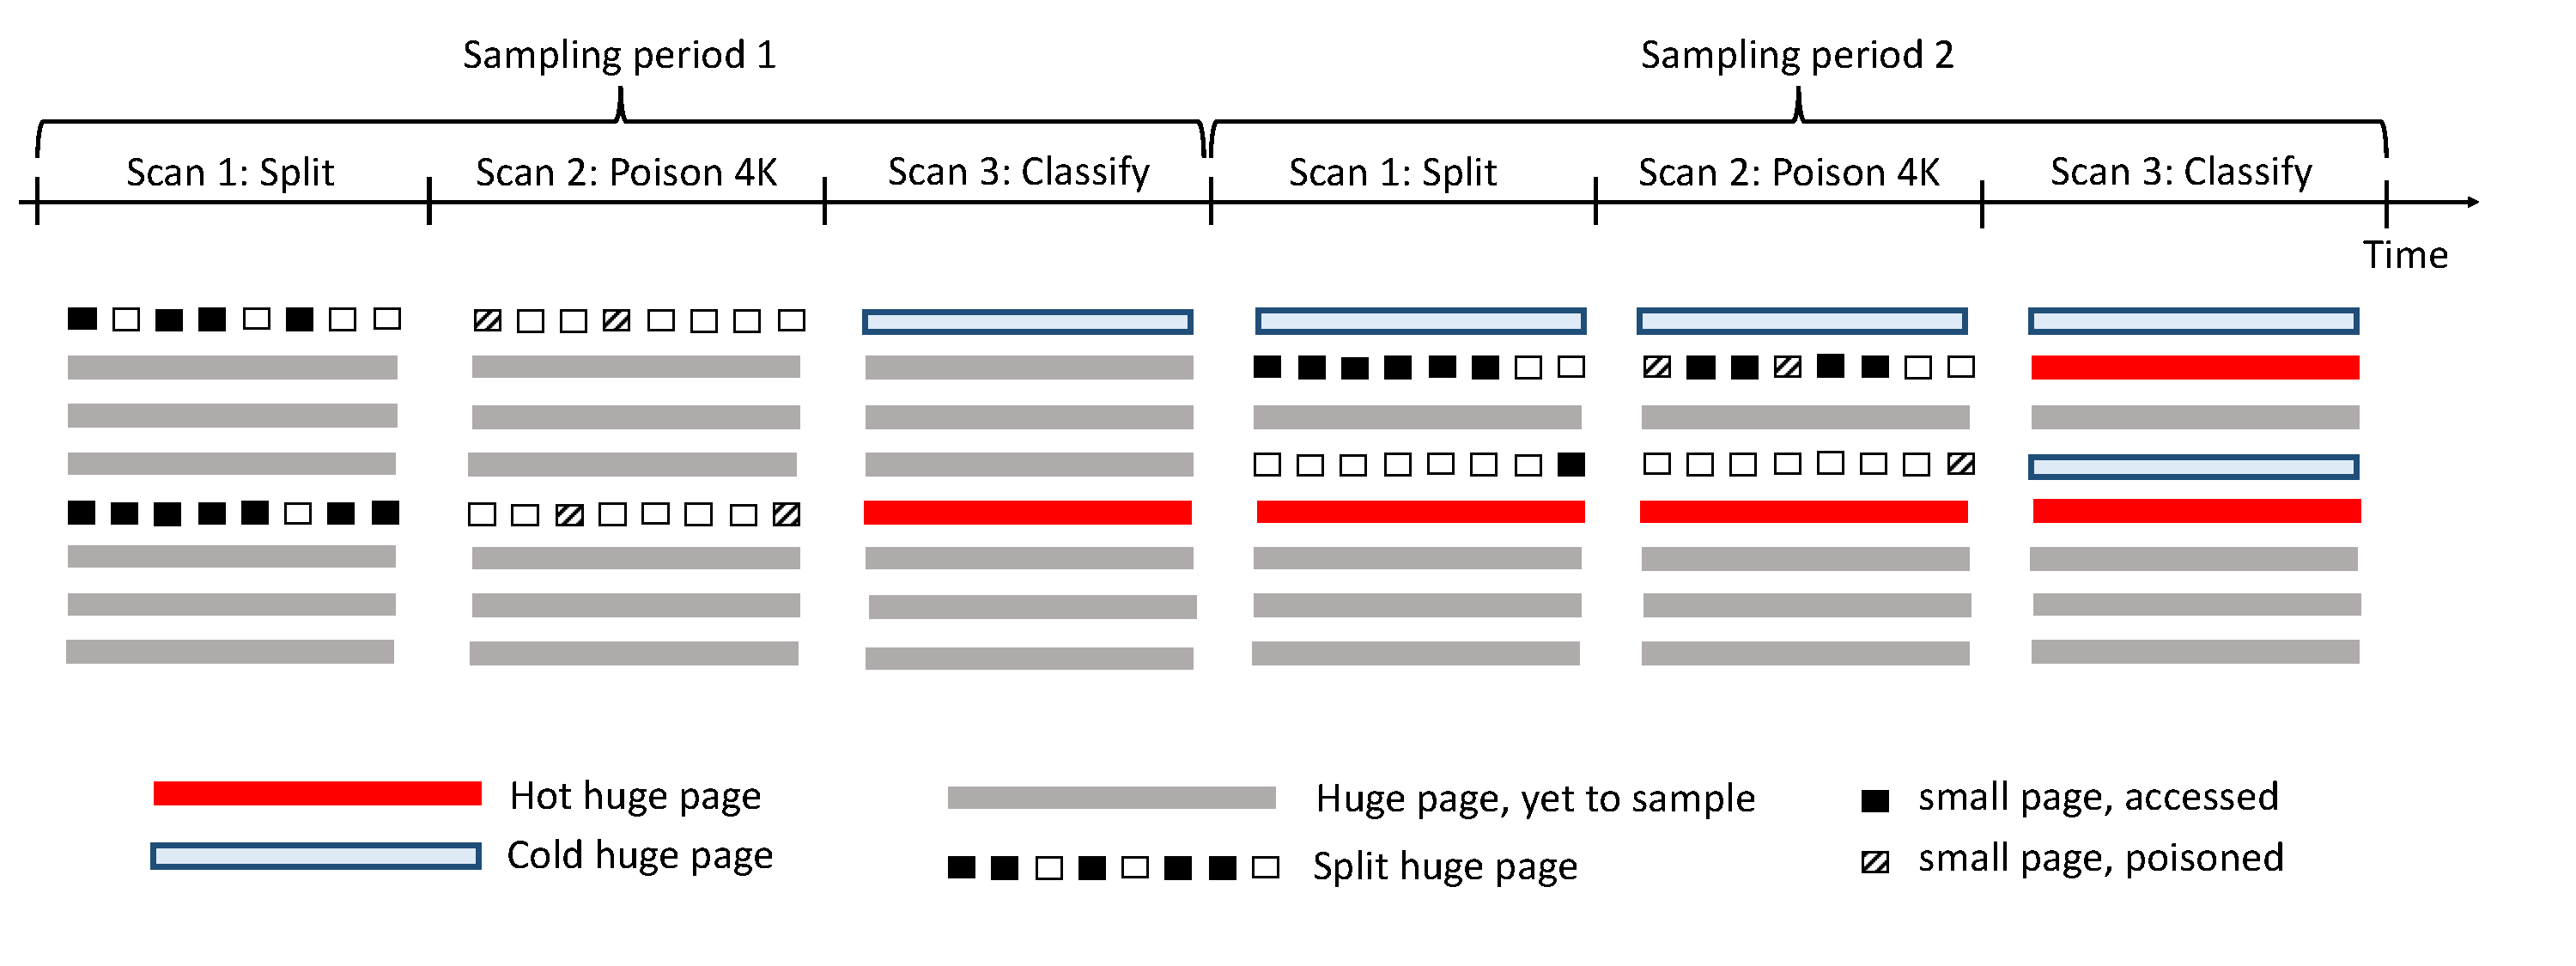
\includegraphics[width=1.0\textwidth]{asplos2017/figures/new-policy-sampling-figure.pdf}
\caption{Thermostat operation: Thermostat classifies huge pages into hot and cold by randomly splitting a
fraction of pages and estimating huge page access rate by poisoning a fraction of 4K
pages within a huge page. The sampling policy is described in
Section~\ref{page-sampling}, Section~\ref{section:access-counting} describes our
approach to page access counting, and Section~\ref{page-classification} describes
the page classification policy. Note that the sampling and poisoning fractions here
are for illustration purposes only. In our evaluation we sample 5\% of huge pages
and poison at most 50 4KB pages from a sampled huge page.}
\label{fig:sampling}
\end{figure*}

\subsection{Overview}
We implement Thermostat in the Linux 4.5 kernel. Thermostat can be controlled at
runtime via the Linux memory control group (cgroup) mechanism~\cite{cgroups}.
All processes in the same cgroup share Thermostat parameters, such as the
sampling period and maximum tolerable slowdown.

The Thermostat mechanism consists of four components: (i) a sampling mechanism
that randomly selects a subset of pages for access rate monitoring, (ii) a monitoring
mechanism that counts accesses to sampled pages while limiting maximum overhead, 
(iii) a classification policy to select pages to place in slow memory, and,
(iv) a mechanism to monitor and detect mis-classified pages or behavior changes and migrate 
pages back to conventional (fast) memory.

The key challenge that Thermostat must address is the difficulty of discerning the access 
rates of 2MB pages at a sufficiently low overhead while still responding rapidly
to changing workload behaviors. Tracking the access rate of a page
is a potentially expensive operation if the page is accessed frequently.  
Hence, to bound the performance impact of
access rate monitoring, only a small fraction of the application footprint may be
monitored at any time.  However, sampling only a small fraction of the application
footprint leads to a policy that adapts only slowly to changes in memory behavior.

\subsection{Page sampling}
\label{page-sampling}
Sampling a large number of huge pages is desirable as it leads to quick
response to time-varying workload access patterns. But, it can lead to a
high performance overhead, since, as explained in
Section~\ref{section:access-counting}, each TLB miss to a sampled page incurs additional
latency for OS fault handling. To tightly control application performance
slowdown, {\it we split a random sample of huge pages (5\% in our case)
into 4KB pages, and poison only a fraction of these 4KB pages in each sampling interval}.
Below, we detail the strategy used to select which 4KB pages to poison, and how
we estimate the total access rate from the access rates of the sampled 4KB
pages.

A simple strategy to select 4KB pages from a set of huge pages is to select $K$
random 4KB pages, for some fixed $K$ ($K = 50$ in our evaluation). However, when only a few 4KB
pages in a huge page are hot, this naive strategy may fail to sample them, and
thus deem the overall huge page to have a low access rate. To address this shortcoming, 
our mechanism monitors page access rates in two steps.
We first rely on the hardware-maintained {\it Accessed} bits to monitor all 512 4KB pages
and identify those with a  non-zero access rate.  We then monitor a sample of these 
pages using our more costly
software mechanism to accurately estimate the aggregate access rate of 
the 2MB page. With our strategy, {\it only 0.5\% of overall 4KB pages are
sampled at any time} -- which makes the performance overhead due to sampling
$<$ 1\%.

To compute the aggregate access rate at 2MB granularity from the access rates of the sampled
4KB pages, we scale the observed access rate in the sample by the total number
of 4KB pages that were marked as accessed. The monitored 4KB pages comprise a 
random sample of accessed pages, while the remaining pages have a negligible
access rate.

\subsection{Page access counting}
\label{section:access-counting}
Current x86 hardware does not support access counting at a per-page granularity.
Thus, we design a software-only solution to track page access rates with very
low overhead ($<$1\%) by utilizing PTE reserved bits. In
Section~\ref{counting_hardware}, we discuss two extensions to existing x86
mechanisms that might enable lower overhead page access counting.

To approximate the number of accesses to a page, we use BadgerTrap, a kernel
extension for intercepting TLB misses~\cite{ref:badgertrap}. When a page is
sampled for access counting, Thermostat poisons its PTE by setting a reserved
bit (bit 51), and then flushes the PTE from the TLB.  The next access to the
page will incur a hardware page walk (due to the TLB miss) and then trigger a
protection fault (due to the poisoned PTE), which is intercepted by BadgerTrap.
BadgerTrap's fault handler unpoisons the page, installs a valid translation in
the TLB, and then repoisons the PTE. By counting the number of BadgerTrap
faults, we can estimate the number of TLB misses to the
page, which we use as a proxy for the number of memory accesses.

Note that our approach assumes that the number of TLB misses and 
cache misses to a 4KB page are similar.  For hot pages, this assertion does not
hold.  However, Thermostat has no need to accurately estimate the access rate
to hot pages; it is sufficient to know that they are hot.  Conversely, for cold pages
nearly all accesses incur both TLB and cache misses as there is no temporal
locality for such accesses, and, therefore, tracking
TLB misses is sufficient to estimate the page access rate. We validated our 
approach by measuring
the TLB miss rates (resulting in page-walks) and last-level cache miss rates for
our benchmark suite using hardware performance counters via the Linux {\tt perf}
utility. For pages we identify as cold, the TLB miss rate is typically higher (but
always within a factor of two) of the last-level cache miss rate measured
without BadgerTrap, indicating that our approach is reasonable.

\subsection{Page classification}
\label{page-classification}
Classifying pages as hot or cold is governed by the user-specified maximum
tolerable slowdown (without such a threshold, one can simply declare all
pages cold and call it a day). To select cold pages, we use the estimated access
rates of each (huge) page.

We translate a tolerable slowdown of $x\%$ to an access rate
threshold in the following way. Given $A$ accesses to slow memory in one second,
the total time consumed by slow memory accesses is $At_s$, where $t_s$ is the
access latency of the slow memory.
Thus, a slowdown threshold of $x\%$ can be translated to an access rate
threshold of $\frac{x}{100t_s}$ per second. If a fraction $f$ of the total
huge pages were sampled, we assign pages to the slow memory such that their
aggregate estimated access rate does not exceed
$f\frac{x}{100t_s}$. We sort the sampled huge pages in increasing
order of their estimated access rates, and then place the coldest pages in slow
memory until the total access rate reaches the target threshold.

This simple approach governs the access rate to slow memory to avoid the
user-specified degradation target. In Figure~\ref{fig:fault-rate}, we
show slow memory access rate averaged over 30 seconds for our benchmark suite,
assuming 1us slow memory access latency and 3\% tolerable slowdown (we discuss
detailed methodology in Section~\ref{section:methodology}). We observe that
Thermostat keeps the slow memory access rate close to the target 30K
accesses/sec. For Aerospike and Cassandra slow memory access rate
temporarily exceeds 30K accesses/sec but is brought back below 30K accesses/sec by 
mis-classification detection, discussed next in
Section~\ref{classification-correction}.

\subsection{Correction of mis-classified pages}
\label{classification-correction}
Since we estimate the access rate of a huge page based on the access rates
of only a few (not more than 50, as described in
Section~\ref{page-sampling}) 4KB pages, there is always some probability
that some hot huge pages will be mis-classified as cold due to sampling error. 
Such mis-classifications are detrimental to application
performance, since the interval between successive samplings of any given
huge page can be fairly long. To address this issue, we track the number of
accesses being made to each cold huge page, using the software
mechanism mentioned in Section~\ref{section:access-counting}.  Since the access
rate to these pages is slow by design, the performance impact of this monitoring is low.
In every sampling period we sort the huge pages in slow memory by their access
counts. All the huge pages in slow memory are migrated back to fast memory which
exceed the cumulative tolerable access rate to slow memory. In addition to the
mis-classified pages we also identify pages that become hot over time, adapting
to the change in application's hot working set.
%A huge page in slow memory is migrated back to fast memory if its actual access rate 
%exceeds its previously estimated access rate. 
%In addition, we do not migrate back a page if its actual rate is less than 50
%accesses/second to prevent thrashing behavior for cold pages with
%unstable access rates.

\begin{figure}[t]
\centering
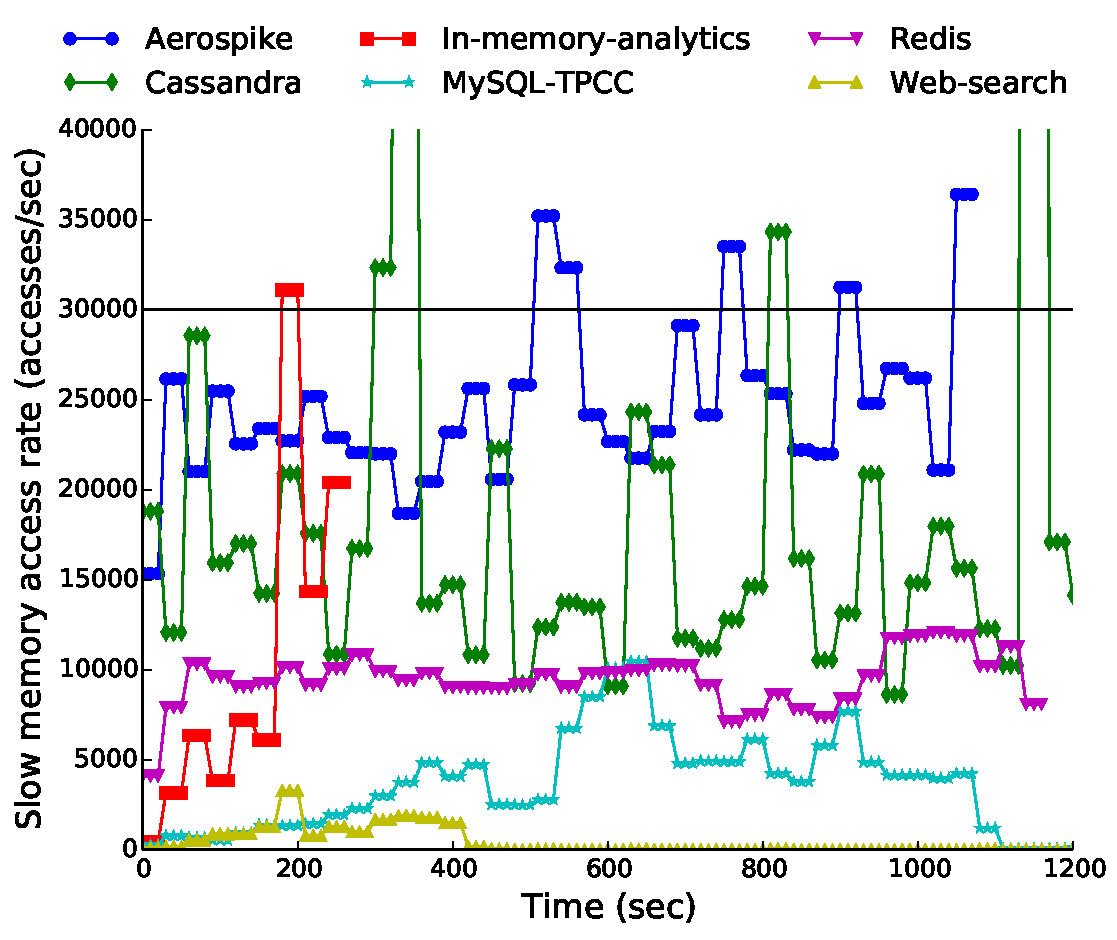
\includegraphics[width=1.0\columnwidth]{asplos2017/figures/faults.pdf}
\caption{Slow memory access rate over time. For a 3\% tolerable slowdown and 1us
slow memory access latency, the target slow memory access rate is 30K accesses/sec.
Thermostat tracks this 30K accesses/sec target. Note that different benchmarks
have different run times; we plot x-axis for 1200 seconds.} 
\label{fig:fault-rate}
\end{figure}

\subsection{Migration of cold pages to slow memory}
Once cold pages have been identified by the guest, they must be migrated to 
the slow memory. We use the NUMA support in KVM guests to achieve this transfer. The NVM
memory space is exposed to the guest OS as a separate NUMA zone, to which the guest
OS can then transfer memory. NUMA support in KVM guests already exists in Linux
and can be used via {\tt libvirt}~\cite{libvirt-numa}.

\subsection{Thermostat example}
Figure~\ref{fig:sampling} illustrates Thermostat's page classification for an
example application with eight huge pages. Each sampling period comprises 
three stages: (i) split a fraction of huge pages, (ii) poison a fraction of split and
accessed 4KB pages, record the access count to 4KB pages to estimate access rate
of the huge pages, and, (iii) classify pages as hot/cold. In this example, we sample 25\% of
huge pages (two huge pages out of eight are sampled). In the first sampling
period, Thermostat splits and records 4KB-grain accesses to two pages (page 1
and 5) in the first scan period. In the second scan period 4KB pages 1 and 4
of the first huge page and 3 and 8 of the fifth huge page are selected to be poisoned.
Thermostat then estimates the access rate to huge page 1 and 5 by from the access rates
of the 4KB pages.  Finally, Thermostat sorts the estimated access rates of the huge pages
and classifies page 1 as cold, as its estimated access rate is below
the threshold tolerable slow memory access rate. However, because the sum of the
access rates of both huge pages is above the threshold access rate, page 5 is classified
as hot. Similarly, in the second sampling period, pages 2 and 4 are randomly
selected for sampling. At the end of the sampling period page 2 is classified as
hot and page 4 as cold.

%\subsection{Linux implementation}
%We implement Thermostat in Linux kernel version 4.5. We add a vector data
%structure using {\tt kmalloc} to track sampled pages storing {\tt struct page}
%pointers and there access rates while sampling.  \fixme{Note that this data
%structure only stores two int type data, hence a low overhead space cost giving
%high returns in overall memory savings.} We split huge pages and merge them in
%place. We piggy back on Linux's {\tt split\_huge\_pmd} functionality to split
%pages and merge small pages back by a custom function similar to {\tt
%khugepaged}'s {\tt collapse\_huge\_page}. We patched in {\tt kstaled} to monitor
%access bit in PTEs~\cite{kstaled}. We use BadgerTrap to poison pages to monitoe
%access rates~\cite{ref:badgertrap}.
%\subsubsection{Thermostat on host system}
%The publicly available version of {\tt kstaled} examines PTEs and PMDs for detecting
%accesses to pages. However, due to reasons discussed in Section~\ref{discussion}, running
%Thermostat on the host is preferable as opposed to in the guest. To use
%Thermostat on
%the host, we modified {\tt kstaled} to examine the accessed bit information in Shadow
%PTEs (SPTE), which is the host page table part of a two-dimensional page table.
%In x86-64, the accessed bits of both PTEs (in guest) and SPTEs (in host) are set
%when a page walk occurs. In case of multiple guests sharing the same physical
%page, the {\tt mmu\_notifier} interface of KVM allows us to go through all the
%VMs in which the page is mapped, and get the accessed information of that page
%by OR-ing the Accessed bits from all the SPTEs.
%
%
%
%Using the Accessed bit, Thermostat can measure whether a page
%was accessed in a given ``scan period'' or not. However, it is difficult to
%judge the hotness of a page based only on a single accessed/not accessed
%outcome. \todo{Also, as we show in Section XXX, a single Accessed bit
%observation can be noisy, and can lead to unnecessary migrations between NVM and
%DRAM.} To solve these problems, we sample the pages for more than one scan
%period. The time period for which pages are sampled is denoted by ``sampling
%period'' (set to 2 scan periods in our experiments). Sampling for multiple scan
%periods allows us to do robust cold page detection, as shown in Section XXX.
%After the sampling period is over, the hugepages are categorized as hot or cold
%by the Thermostat policy outlined next.
%
%
%
%
%\textbf{Page Cache:}Interaction of Kstaled mechanism with unmapped pages,
%e.g., page cache: \todo{Say something here.}
%
%
%\subsection{Translation Facades}
%Second, the Thermostat controller needs an effective mechanism for chunking up a DRAM
%huge page into several small pages, and also for compacting several small hot
%pages into a single DRAM huge page. Chunking up a huge page is relatively simple
%-- one need only allocate several page table entries (PTEs) corresponding to the
%chunked up page. Doing the inverse, that is compacting several small pages from
%the slow-mem and DRAM into a single DRAM huge page has more challenges. First,
%due to memory fragmentation, it may not be possible to find a suitable space to
%put the newly created huge page. Second, reading several small pages from
%slow-mem, and creating a huge page out of them can be a potentially very long
%latency operation, which can then affect application throughput as well as tail
%latency. We plan to study the design trade-off space of when to perform
%these operations and incorporate the obtained insights into building the Thermostat
%controller.
